\section*{\nr.4 \titfour (10 Punkte)}
\begin{enumerate}[(a)]
\item Durch Verwendung von charakteristischen Funktionen lässt sich die Transparenzfunktion $a$ folgendermaßen ausdrücken:
\begin{equation}
a(x,y) = \chi_{(-\infty,\infty)} (y) \left(\chi_{[9d,10d]}(x) + \chi_{[-10d,-9d]}(x) \right)
\end{equation}
Da sich die Funktion in Faktoren von $x$ und Faktoren von $y$ ausdrücken lässt und weil die $y$-Richtung eine Symmetrie auszeichnet, lässt sich das Problem auf eine Dimension reduzieren. Für die Feldstärke in der Beugungsebene gilt also:
\begin{equation}
E(k_x,k_y) \propto \int_\mathbb{R} \mathrm{d}x \left(\chi_{[9d,10d]}(x) + \chi_{[-10d,-9d]}(x) \right)\exp(-ik_x x)
\end{equation}
Folgende leicht zu zeigende Identität möchten wir gleich benutzen:
\begin{equation}
\int_{-\epsilon}^{+\epsilon}\mathrm{d}\mu\exp(-it\mu) = \frac{2}{t}\sin(\epsilon t)
\label{eq:ident}
\end{equation}
Berechnen wir zunächst das Fourierintegral von oben:
\begin{align}
&\int_\mathbb{R} \mathrm{d}x \left(\chi_{[9d,10d]}(x) + \chi_{[-10d,-9d]}(x) \right)\exp(-ik_x x) \\
&= \int_{-10d}^{-9d}\mathrm{d}x\exp(-ik_x x) +\int_{9d}^{10d}\mathrm{d}x\exp(-ik_x x) \\
&= \int_{-10d}^{10d}\mathrm{d}x\exp(-ik_x x) -\int_{-9d}^{9d}\mathrm{d}x\exp(-ik_x x) \\
&= \frac{2}{k_x} \left[ \sin(10k_x d) - \sin(9k_x d) \right]
\end{align}
Dabei wurde im letzten Schritt \vref{eq:ident} verwendet.
Für das gesuchte Beugungsbild gilt also:
\begin{equation}
I(k_x,k_y) \propto \frac{\left[ \sin(10k_x d) - \sin(9k_x d) \right]^2}{k_x^2}
\end{equation}
Der Graph ist in \vref{fig:fourier} veranschaulicht. 
\begin{figure}[htbp]
\centering
% GNUPLOT: LaTeX picture with Postscript
\begingroup
  \makeatletter
  \providecommand\color[2][]{%
    \GenericError{(gnuplot) \space\space\space\@spaces}{%
      Package color not loaded in conjunction with
      terminal option `colourtext'%
    }{See the gnuplot documentation for explanation.%
    }{Either use 'blacktext' in gnuplot or load the package
      color.sty in LaTeX.}%
    \renewcommand\color[2][]{}%
  }%
  \providecommand\includegraphics[2][]{%
    \GenericError{(gnuplot) \space\space\space\@spaces}{%
      Package graphicx or graphics not loaded%
    }{See the gnuplot documentation for explanation.%
    }{The gnuplot epslatex terminal needs graphicx.sty or graphics.sty.}%
    \renewcommand\includegraphics[2][]{}%
  }%
  \providecommand\rotatebox[2]{#2}%
  \@ifundefined{ifGPcolor}{%
    \newif\ifGPcolor
    \GPcolortrue
  }{}%
  \@ifundefined{ifGPblacktext}{%
    \newif\ifGPblacktext
    \GPblacktextfalse
  }{}%
  % define a \g@addto@macro without @ in the name:
  \let\gplgaddtomacro\g@addto@macro
  % define empty templates for all commands taking text:
  \gdef\gplbacktext{}%
  \gdef\gplfronttext{}%
  \makeatother
  \ifGPblacktext
    % no textcolor at all
    \def\colorrgb#1{}%
    \def\colorgray#1{}%
  \else
    % gray or color?
    \ifGPcolor
      \def\colorrgb#1{\color[rgb]{#1}}%
      \def\colorgray#1{\color[gray]{#1}}%
      \expandafter\def\csname LTw\endcsname{\color{white}}%
      \expandafter\def\csname LTb\endcsname{\color{black}}%
      \expandafter\def\csname LTa\endcsname{\color{black}}%
      \expandafter\def\csname LT0\endcsname{\color[rgb]{1,0,0}}%
      \expandafter\def\csname LT1\endcsname{\color[rgb]{0,1,0}}%
      \expandafter\def\csname LT2\endcsname{\color[rgb]{0,0,1}}%
      \expandafter\def\csname LT3\endcsname{\color[rgb]{1,0,1}}%
      \expandafter\def\csname LT4\endcsname{\color[rgb]{0,1,1}}%
      \expandafter\def\csname LT5\endcsname{\color[rgb]{1,1,0}}%
      \expandafter\def\csname LT6\endcsname{\color[rgb]{0,0,0}}%
      \expandafter\def\csname LT7\endcsname{\color[rgb]{1,0.3,0}}%
      \expandafter\def\csname LT8\endcsname{\color[rgb]{0.5,0.5,0.5}}%
    \else
      % gray
      \def\colorrgb#1{\color{black}}%
      \def\colorgray#1{\color[gray]{#1}}%
      \expandafter\def\csname LTw\endcsname{\color{white}}%
      \expandafter\def\csname LTb\endcsname{\color{black}}%
      \expandafter\def\csname LTa\endcsname{\color{black}}%
      \expandafter\def\csname LT0\endcsname{\color{black}}%
      \expandafter\def\csname LT1\endcsname{\color{black}}%
      \expandafter\def\csname LT2\endcsname{\color{black}}%
      \expandafter\def\csname LT3\endcsname{\color{black}}%
      \expandafter\def\csname LT4\endcsname{\color{black}}%
      \expandafter\def\csname LT5\endcsname{\color{black}}%
      \expandafter\def\csname LT6\endcsname{\color{black}}%
      \expandafter\def\csname LT7\endcsname{\color{black}}%
      \expandafter\def\csname LT8\endcsname{\color{black}}%
    \fi
  \fi
    \setlength{\unitlength}{0.0500bp}%
    \ifx\gptboxheight\undefined%
      \newlength{\gptboxheight}%
      \newlength{\gptboxwidth}%
      \newsavebox{\gptboxtext}%
    \fi%
    \setlength{\fboxrule}{0.5pt}%
    \setlength{\fboxsep}{1pt}%
\begin{picture}(7936.00,3400.00)%
    \gplgaddtomacro\gplbacktext{%
      \csname LTb\endcsname%
      \put(814,704){\makebox(0,0)[r]{\strut{}$0$}}%
      \put(814,1146){\makebox(0,0)[r]{\strut{}$0.2$}}%
      \put(814,1588){\makebox(0,0)[r]{\strut{}$0.4$}}%
      \put(814,2030){\makebox(0,0)[r]{\strut{}$0.6$}}%
      \put(814,2472){\makebox(0,0)[r]{\strut{}$0.8$}}%
      \put(814,2914){\makebox(0,0)[r]{\strut{}$1$}}%
      \put(1707,484){\makebox(0,0){\strut{}$-10$}}%
      \put(2975,484){\makebox(0,0){\strut{}$-5$}}%
      \put(4243,484){\makebox(0,0){\strut{}$0$}}%
      \put(5510,484){\makebox(0,0){\strut{}$5$}}%
      \put(6778,484){\makebox(0,0){\strut{}$10$}}%
    }%
    \gplgaddtomacro\gplfronttext{%
      \csname LTb\endcsname%
      \put(176,1919){\rotatebox{-270}{\makebox(0,0){\strut{}$I/I_0$}}}%
      \put(4242,154){\makebox(0,0){\strut{}$d\cdot k_x$}}%
    }%
    \gplgaddtomacro\gplbacktext{%
      \csname LTb\endcsname%
      \put(814,704){\makebox(0,0)[r]{\strut{}$0$}}%
      \put(814,1146){\makebox(0,0)[r]{\strut{}$0.2$}}%
      \put(814,1588){\makebox(0,0)[r]{\strut{}$0.4$}}%
      \put(814,2030){\makebox(0,0)[r]{\strut{}$0.6$}}%
      \put(814,2472){\makebox(0,0)[r]{\strut{}$0.8$}}%
      \put(814,2914){\makebox(0,0)[r]{\strut{}$1$}}%
      \put(1707,484){\makebox(0,0){\strut{}$-10$}}%
      \put(2975,484){\makebox(0,0){\strut{}$-5$}}%
      \put(4243,484){\makebox(0,0){\strut{}$0$}}%
      \put(5510,484){\makebox(0,0){\strut{}$5$}}%
      \put(6778,484){\makebox(0,0){\strut{}$10$}}%
    }%
    \gplgaddtomacro\gplfronttext{%
      \csname LTb\endcsname%
      \put(176,1919){\rotatebox{-270}{\makebox(0,0){\strut{}$I/I_0$}}}%
      \put(4242,154){\makebox(0,0){\strut{}$d\cdot k_x$}}%
    }%
    \gplbacktext
    \put(0,0){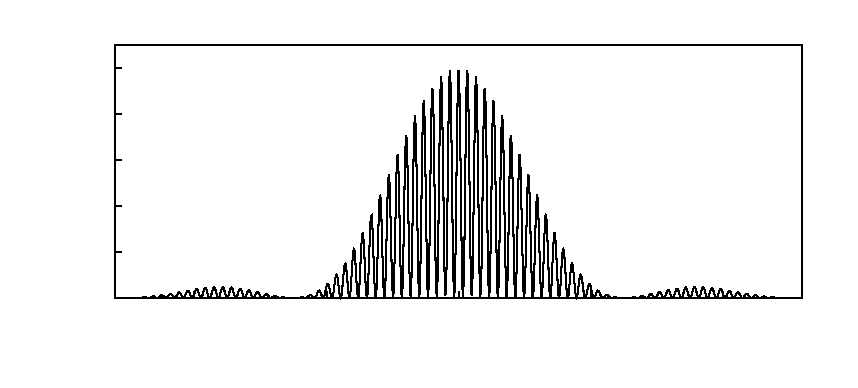
\includegraphics{beugung}}%
    \gplfronttext
  \end{picture}%
\endgroup

\caption{Beugungsbild für beliebiges festes $k_y$ in Einheiten von $d\cdot k_x$.}
\label{fig:fourier}
\end{figure}

\item \vref{fig:fourier} zeigt einen schnell und einen langsam oszillierenden Anteil. Dabei verursacht die Beugung am jeweiligen Einzelspalt den schnell oszillierenden Anteil, während der langsam oszillierende Anteil daher rührt, dass Interferenz zwischen den beiden Spalten stattfindet.

\item Sei $\tilde{I}(k_x,k_y)$ diejenige Intensität, die in der Beugungsebene ankäme, wenn kein Beugungsobjekt vorhanden wäre. Da das Licht parallel einfällt und kohärent ist, gilt $\tilde{I}(k_x,k_y) \equiv \tilde{I}_0$ konstant. Für das inverse Beugungsmuster gilt dann:
\begin{equation}
I^{-1} (k_x,k_y) = \tilde{I}_0 - I (k_x,k_y)
\end{equation}
Das Muster in \vref{fig:fourier} wäre also an der $x$-Achse gespiegelt und in positive $I$-Richtung verschoben.

\end{enumerate}